\chapter{Robust and GPU-friendly Isotropic Meshing Based on Narrow-banded Euclidean Distance Transformation}


\section{Overview}
  In this paper, we propose a simple-yet-effective method for isotropic meshing via Euclidean distance transformation based Centroidal Voronoi Tessellation (CVT).
  The proposed approach aims at improving the performance as well as robustness of computing CVT on curved domains
  while simultaneously maintaining the high-quality of the output meshes.
  In contrast to the conventional extrinsic methods which compute CVTs in the entire volume bounded by the input model,
  our idea is to restrict the computation in a 3D shell space with user-controlled thickness.
  Taking the voxels which contain the surface samples as the sites, we compute the exact Euclidean distance transform on the GPU.
  Our algorithm is fully parallel and memory-efficient,
  and it can construct the shell space with resolution up to $2048^3$ at interactive speed.
  Since the shell space is able to bridge holes and gaps up to a certain tolerance, and tolerate non-manifold edges and degenerate triangles,
  our algorithm works well on models with such defects, whereas the conventional remeshing methods often fail.

%-------------------------------------------------------------------------
\section{Introduction}

  Triangle meshes have found widespread acceptance in computer graphics as a simple, convenient, and versatile representation of surfaces.
  However, raw meshes obtained from 3D scanners are often not ready for subsequent geometric processing,
  since they may contain holes, gaps, noise, degenerate triangles and non-manifold edges.

  A popular approach to improve the mesh quality is via centroidal Voronoi tessellation (CVT),
  which can generate a highly regular distribution of sites with respect to a given density function.
  A typical CVT-based remeshing method iteratively updates the generator of each Voronoi cell
  until it coincides with its center of mass.
  Then the isotropic mesh is obtained by the dual graph of the computed CVT.
  A key step in CVT computation is to construct Voronoi diagrams (VD) in each iteration.
  Although it is fairly simple to construct VD in Euclidean spaces,
  computing VD on curved domains is expensive due to lack of closed-form formula of geodesic distance.
  A practical way is to compute the restricted Voronoi diagrams (RVD)~\cite{DBLP:journals/cgf/YanLLSW09},
  which is the intersection between the given model and a CVT defined in $\mathbb{R}^3$.

  In this paper, we propose a new RVD-based computational framework for isotropic meshing,
  aiming at improving the performance as well as robustness of computing RVD
  while simultaneously maintaining the high-quality of output meshes.
  Rather than computing CVTs in the entire volume bounded by the input model,
  our idea is to restrict the computation in a 3D shell space with user-controlled thickness.
  Since the shell space is able to bridge holes and gaps up to a certain tolerance,
  and also tolerate non-manifold edges and degeneracies, our algorithm works well on imperfect meshes with such defects,
  whereas the conventional \textit{remeshing} methods often fail. See Figure~\ref{fig:ami_broken}.

  \begin{figure}[thb]
  \centering
  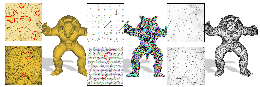
\includegraphics[width=0.9\textwidth]{figs/gcvt/ami_broken}\\
  \begin{scriptsize}
  \makebox[0.95in]{Input mesh} \makebox[0.950in]{CVT} \makebox[0.950in]{Dual triangulation}
  \end{scriptsize}
  \vspace{-0.1in}
  \caption{Isotropic meshing on an imperfect mesh with non-manifold edges, degenerate triangles and holes.}
  \label{fig:ami_broken}
  \end{figure}

  This paper makes the following contributions:
  \begin{itemize}
  \item We propose an efficient framework for constructing isotropic meshes via voxel representation.
  It can completely avoid the computationally expensive components,
  such as implicit function fitting, isosurface extraction, and geodesic distance computation, which are often used in the existing methods.
  \item Our framework can produce topologically consistent shell space with user control
  so that it can bridge holes and gaps and tolerate noise to some certain extent.
  It also works well for models with non-manifold edges and degenerate triangles.
  \item We present a fast and memory-efficient algorithm for computing narrow-banded distance fields on GPUs.
  The CVT, RVD and the dual Delaunay triangulations are also computed in parallel on the GPUs.
  \end{itemize}

%-------------------------------------------------------------------------

\vspace{-0.3cm}



  \begin{figure}[t]
  \centering
  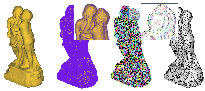
\includegraphics[width=0.8\textwidth]{figs/gcvt/sculpture}
  \vspace{-0.2in}
  \caption{Overview of our approach on the Sculpture model.
  (a) Input mesh; (b) Shell space with $d=3$; (c) CVT with 3K seeds;
  (d) The output isotropic mesh.
  }
  \label{fig:scuplture}
  \end{figure}

%-------------------------------------------------------------------------
\vspace{-0.4cm}

\section{Algorithm}
\label{sub:algorithm}
  Let $O$ denote the input 3D mesh.
  We first construct a voxel representation $M$ of $O$ at a given resolution $res$.
  Then we construct a shell space $\bar{P}$ consisting of off-surface points,
  where each point in $\bar{P}$ has a distance $d_p\leq d$ to its closest point on $M$.
  The threshold $d$ is specified by the user and model-dependent.

  Our isotropic meshing algorithm adopts Lloyd's framework.
  Starting with $k$ randomly generated seeds, it minimizes the CVT energy by iteratively updating the seed positions.
  In each iteration, it computes the Voronoi diagrams confined in the shell space and moves the seeds toward the corresponding mass centers.
  The algorithm projects the seeds back to $\bar{P}$ if they are outside the shell space.
  Upon convergence, it propagates the seed information in the shell space to look for connected Voronoi cells and extracts the dual Delaunay triangulation.
  Our method is described in detail in the next subsections, and furthermore outlined in Algorithm~\ref{ALGORITHM:meshing}.

  \begin{algorithm}
  \caption{Isotropic Meshing based on EDT}\label{ALGORITHM:meshing}
  \renewcommand{\algorithmicrequire}{\textbf{Input:}}
  \renewcommand{\algorithmicensure}{\textbf{Output:}}
  \begin{algorithmic}[1]
  \Require 3D surface $O$, voxel resolution $res$, shell space thickness $d$, convergence threshold $\epsilon$, and number of seeds $k$
  \Ensure Isotropic mesh with $k$ vertices
  \State $S \gets k$ random seeds
  \State $M$ $\gets$ Voxelization($O$, $res$)
  \State $\bar{P}$ $\gets$ ShellSpaceConstruction($M$, $res$, $d$)
  \While {convergence not reached}
  \State $V_k$ $\gets$ SearchClosestSeedInShell($\bar{P}$, $S$)
  \State $C_k$ $\gets$ CenterMass($V_k$)
  \State $\bar{C}_k$ $\gets$ UpdateSeed($\bar{P}$, $C_k$)
  \State $S$ $\gets$ $\bar{C}$
  \EndWhile
  \State $V_k$ $\gets$ ShellFlooding($\bar{P}$, $S$)
  \Return DualTriangulation($V_k$)
  \end{algorithmic}
  \end{algorithm}

%------------------------------------------------------------------------
\vspace{-0.4cm}

\subsection{Memory-efficient Shell Space Construction}
\label{sub:Shell Space Computation}
  We introduce a memory-efficient way to construct shell spaces in real-time.
  We extend the Parallel Banding Algorithm (PBA) of Cao et al.~\cite{Cao:2010} to compute Euclidean distance transform (EDT) in the narrow-band manner.
  Their algorithm partitioned the input domain into small chunks of equal size, which can be processed in parallel.
  The results are then merged concurrently.
  Although their method is exact and efficient, it is not practical for large-scale models due to rapidly growing memory consumption.
  Our method addresses this memory issue by on-the-fly computation and integrating fast bitmap indexing technology on GPUs.
  We explain the principle in two dimensions for simplicity; the idea can be easily extended to three dimensions.

  The input image is divided into a virtual grid made up of occupied and non-occupied pixels,
  where the former pixels, denoted as sites $\in S$, are run-length encoded.
  Every pixel goes through a two-step process : (1) finding the nearest site $S_{ij}$, among all sites in row $j$;
  (2) determining the closest site, among all the nearest sites in the current column $i$.
  For the first step we assign one thread to process a row because it's more efficient to do more computation in a single thread
  than repeatedly accessing global memory with multiple threads.
  The second step extends the dividing-and-merging approach of PBA,
  with employing warp\footnote{A warp is a pool of threads that executes physically in parallel.}-vote and warp-shuffle functions in CUDA to exchange the nearest sites information within a chunk.
  We make every thread in the same warp doing the same calculation,
  hence greatly reducing the warp variation that often compromises performance.

   \begin{figure}[ht]
  \centerline{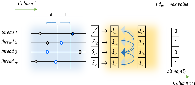
\includegraphics[width=0.8\textwidth]{figs/gcvt/distanceField2}}
  \vspace{-0.1in}
  \caption{An illustrative example on distance field computation in a narrow band.
  See the text for the description and function \emph{ShellSpaceConstruction} for the pseudo code.
  }
  \label{fig:DF}
  \end{figure}

  \begin{algorithm}
  \label{ALGORITHM:shellspace}
  \begin{algorithmic}
  \State \textcolor[rgb]{0, 0.5, 0}{// \emph{To ease representation, we show the 2D version here}}
  \State \textbf{function} ShellSpaceConstruction($M, res, d$)
  \ForAll {\textbf{thread} $j = 0$~to~$res$ \textbf{in} $parallel$}
        \For {$i = 0~\textbf{to}~res$}
            \State $S_{ij} \leftarrow  \emph{GetNearestSite}($M$, $$, $j$, $d$)$
            \State \textbf{discard} $S_{ij}$ \textbf{if} $\parallel d_{ij} \parallel > d$
            \State \textbf{set barrier} \textcolor[rgb]{0.00,0.50,0.00}{// \emph{Ensure every thread gets $S_{ij}$}}
            \State \textcolor[rgb]{0.00,0.50,0.00}{// \emph{Compare with other threads in same warp}}
            \State \textcolor[rgb]{0.00,0.50,0.00}{// \emph{warp size = h, current warp ID = k}}
            \State $C_{k}$ $\gets$ $S_{ij}$ %\textcolor[rgb]{0.00,0.50,0.00}{// \emph{current warp ID = k}}
            \For {$x$ = $0$ \textbf{to} $h$} %\textcolor[rgb]{0.00,0.50,0.00}{// \emph{warp size = h}}
                \If {\emph{ IsCloser}($C_k$, $C_x$)}
                        \State $C_{k}$ $\gets$ $C_{x}$
                        \State $id \gets x$
                \EndIf
            \EndFor
            \State \textcolor[rgb]{0.00,0.50,0.00}{// \emph{Mark the closest site of pixel ($i,j$) }}
            \State $Bitmap[i][id] = true$
        \EndFor
  \EndFor
  \State Collect and merge the closest sites if $Bitmap[i][j]$ = true
  \State \textbf{return} $\bar{P}$ \textcolor[rgb]{0.00,0.50,0.00}{// \emph{return pixels located inside the shell}}
  \end{algorithmic}
  \end{algorithm}


  Let's take Fig.~\ref{fig:DF} as an example.
  When the threads in a warp come to column $i$, each row will compute their corresponding nearest sites $S_{ij}$.
  The nearest site of the current pixel is colored in blue.
  Note that only some sites (Blue-blank dots) satisfy the the distance constraint.
  Therefore, the sites $S_{i1}$ of thread 1 can be safely discarded.
  We set a barrier to ensure that every thread obtains some sites before exchanging information.
  After synchronization, we sweep each $S_{ij}$ to other threads in the same warp to update the closest site of the current pixel ($i$,$j$),
  based on the distance function $d_{ij}$.
  A bitmap stores a key (boolean) value for every pixel.
  The '0's indicate that the corresponding nearest sites are \textbf{not} possible to be the closest sites of the current column.
  Then the threads repeat the same procedure for the next column $i+1$ until they reach the last column.
  In the final step we collect the closest sites with flag '1' in different chunks and merge them to get the pixels that form the shell region.
  Since the nearest sites are computed on-the-fly and the temporary result is indexed by bitmap only,
  our algorithm requires less memory than the PBA method.

%-------------------------------------------------------------------------

\vspace{-0.4cm}

\subsection{Constructing 3D Voronoi Diagrams in Shell Space}
\label{sec:RVD}
  As mentioned above, the shell space represented by $\bar{P}$ is used as constraints to construct Voronoi diagrams and update the positions of seeds.
  Initially, the seeds $S$ = $\{s_1,..,s_k\}$ are located on the input mesh.
  We collect points $\in \bar{P}$ that share the same closest seeds to build Voronoi diagrams.

  We perform a proximity search to find the closest seed for all query points from $\bar{P}$.
  To speed up the process, the seeds are projected onto a uniform grid $G$ with smaller resolution of $res$ (e.g. $32^3$), such that,
  for a query point $q$, it just looks up the seeds in the grid cell $G_q$ where $q$ falls into.
  In case any border of the grid cell is closer to $q$ than the seed found in $G_q$, query point $q$ looks up the neighbor cell of $G_q$.

\vspace{-0.4cm}

\subsection{Computing CVTs}
\label{sec:RCVT}

   Updating the seeds' position towards uniform distribution is crucial for constructing CVT.
   Based on the following energy function, optimal positions can be reached by minimizing $E(S)$.

  \vspace{-0.8cm}

  \begin{displaymath}
  E(S) = \sum \limits_{i=1}^m \; \int_{V_i}\rho (\mathit{p}) \|\mathit{p}-s_i\|^2 \mathit{d}\mathit{p},%{{ln}} \left[ \frac{ \phi(t-\tau) }{ \bar{\phi} } \right],
  \end{displaymath}
  where $V_i$ is the Voronoi cell of seed $s_i$, $p$ $\in \bar{P}$ and  $\rho$ is a non-negative user-defined density function.

  According to Lloyd's algorithm, a seed $s_i$ moves iteratively toward the corresponding mass center $c_i$ of Voronoi Diagram $V_i$ until convergence.
  However, the mass center could be located far from the surface, as is constructed in the shell space.
  We consider the following new position to replace mass center for each iteration.

  \vspace{-0.5cm}
  \begin{displaymath}
  \bar{c}_i = s_i + u\frac{\protect \overrightarrow{s_ic_i}}{\|\protect \overrightarrow{s_ic_i}\|},
  \end{displaymath}
  where $u\in\mathbb{R}^{+}$ is the magnitude of movement of seeds.
  We observed that if the seeds move in different magnitude, the area of CVTs will largely vary depending on surface curvature.
  In addition, in order to guarantee the topology consistence, the new center will be projected back to $M$ if it exceeds the shell space, as shown in Fig.~\ref{fig:centroid_movement}.

\begin{figure}[tbh]
  \centering
  \includegraphics[width=1.0\linewidth]{figs/gcvt/centroid}
  \begin{scriptsize}
  \makebox[1.55in]{(a)}\makebox[1.55in]{(b)}\\
  \end{scriptsize}
  \vspace{-0.1in}
  \caption{Illustration of the update process with two seeds in an iteration.
  (a) Yellow dots are the seeds of Voronoi cells $V_i$ (in red) and $V_j$ (in green).
  Red and green dots are their mass centers respectively.
  (b) The seeds move along vector $\protect \overrightarrow{sc}$ to the new centers (blue dots).
  Project $\bar{c}_j$ (light blue dot) to the surface since it is outside the shell region.
  }
  \label{fig:centroid_movement}
  \end{figure}
%-------------------------------------------------------------------------

%-------------------------------------------------------------------------
\vspace{-0.5cm}

\subsection{Computing Dual Triangulations}
\label{sec:MeshExtraction}

  Upon convergence we have all the generators uniformly distributed.
  The remain part describes how to extract the dual Delaunay triangulation.

  First, we find the direct neighbors of all seeds, where the direct means if there exists two voxels from their Voronoi cells that are connected.
  The adjacency neighbors can be found by flooding all seeds information to all voxels in the shell $\in \bar{P}$.
  Each voxel associates a hash table to hold the location of neighbors (26 voxels).
  Each propagation updates the current seed information to neighbor voxels until all voxels are reached.
  This approach avoids producing wrong network for seeds that are geometrically close, but topologically far from each other.
  After that we organize their direct neighbors in clockwise order and finally extract the triangle mesh.

\vspace{-0.4cm}

%-------------------------------------------------------------------------
\section{Experimental Results}
\label{sec:results}
  All tests were performed on a PC with an Intel Xeon E5 2.5GHz CPU and an nVidia Quadro K5000 with 4GB RAM.

\vspace{-0.4cm}

\subsection{Narrow-banded Distance Fields}
\label{sec:results_DF}
  Table \ref{tab:DFtable} lists the computational time and the peak memory under varying parameter $d$ and $res$ (~Fig.\ref{fig:Shell space comparison}).
  Clearly, when $d$ increases,
  the computational time increases insignificantly with the increased amount of nearest sites in the shell.
  This is due to the low cost of intra-warp communication and the reduction of warp divergence in our algorithm.
  Also, the memory consumption is remarkably small, considering the scene is in high resolution uniform grid.
  Traditional algorithms (e.g.,~\cite{Cao:2010}) usually require memory at least 10 times more than ours.

\begin{table}[tbh]
\caption{Performance (time in seconds) of our algorithm on different $d$ in resolution $1024^3$ and $2048^3$.}
\begin{center}
\begin{tabular}{lclclcllclcllcl}
\hline
    Model & $d$ & Memory & Time & Memory & Time \\
 \hline
   Dinosaur  & 1  & 149MB  &   1.186 & 1.18GB & 12.3  \\
             & 3  & 174MB  &   1.239 & 1.23GB & 13.1\\
             & 6  & 206MB  &  1.313 & 1.30GB  & 13.3\\
             & 9  & 235MB  &  1.383 & 1.36GB & 13.5 \\

  \hline
\end{tabular}
\end{center}
\label{tab:DFtable}
\end{table}


  Table \ref{tab:PBAtable} compares our algorithm with PBA on the Sculpture model in resolution $512^3$.
  Since PBA computes a full distance map, their performance is independent of distance $d$.
  The result shows that our algorithm consumes significantly less memory and runs much faster than PBA with a reasonably small $d$.

\begin{table}[tbh]
\caption{Comparison of our algorithm with PBA in resolution $512^3$ (time in seconds).}
\begin{center}
\begin{tabular}{lclclclcl}
\hline
    Model & Memory & $d$ & Time \\
 \hline
 Sculpture (PBA) & 1073MB    & N/A    &   0.310   \\
 Sculpture (Ours)  & 26.6MB    & 1    &   0.147($\times$2.1)  \\
             & 33.7MB    & 3    &   0.173 ($\times$1.8) \\
             & 49.7MB    & 6    &  0.200 ($\times$1.6) \\
             & 66.1MB    & 15    &  0.286 ($\times$1.1) \\
             & 76.2MB    & 20      & 0.339($\times$0.9) \\

  \hline
\end{tabular}
\end{center}
\label{tab:PBAtable}
\end{table}


\begin{figure*}[tbh]
\centerline{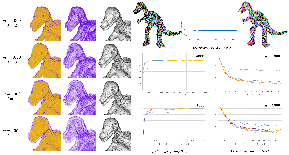
\includegraphics[width=\linewidth]{figs/gcvt/bandComparison-horizontal2}}
\vspace{-0.15in}
\caption{Evaluating the mesh quality under various shell space parameter $d$.
(a) and (b) show the triangulation quality measure and the singularity ratio.
(c) We also observe that our GPU-based Lloyd algorithm converges in usually 100-200 iterations
and $d$ has little impact on the convergence rate.
The horizontal axis shows the iteration number and the vertical axis is the normalized CVT energy function.
}
  \label{fig:Shell space comparison}
\end{figure*}

\vspace{-0.5cm}
%------------------------------------------------------------------------
\subsection{CVT Computation}
\label{sec:results_CVT}
  Similar to~\cite{DBLP:journals/cad/WangYLXWGM015}, we adopted the following criteria to measure the triangle mesh quality.
  (1) Triangle quality $Q(t)$ defined by ${6P_{t}}/{\sqrt{3}H_{t}}$, where $P_t$ and $H_t$ are the inradius and the length of the longest edge of triangle $t$.
  (2) The smallest angle $\theta _{min}$ and the average $\theta _{avg}$ of minimal angles of all triangles.
  (3) The ratio of singularities, defined by $v_s / k$, where $v_s$ is the number of non 6-valent vertices and $k$ is the number of vertices.

   We allow the user to balance accuracy and efficiency in the choice of offset $d$.
   Figure \ref{fig:Shell space comparison} describes the relationship between the distance $d$, the number of generator and the quality of remeshed surface.
   As the offset increases to $9$, with 4k generators, the mesh quality of dinosaur model dramatically drops.
   This also happens when the offset decreases to $2$ with 1k generators.
   Figure \ref{fig:Shell space comparison}(b) illustrates the quality difference between different $d$ clearly.
   Along with other examples in Table \ref{tab:Performancetable}, we can show that the mesh is at best quality with offset distance in specified range (2 to 6).
   Figure \ref{fig:OursRVDGVD} compares our method with two parameterization-free isotropic meshing methods,
   the \textit{intrinsic} CVT method by Wang et al~\cite{DBLP:journals/cad/WangYLXWGM015}
   and the \textit{extrinsic} RVD method by Yan et al.~\cite{DBLP:journals/cgf/YanLLSW09}.
   Thanks to the GPU-friendly structure and the computational power of modern GPUs,
   our method runs significantly faster than their CPU-based implementations.

\begin{figure}[tbh]
\centering
\begin{scriptsize}
\makebox[0.3\textwidth]{\textbf{Ours}}
\makebox[0.3\textwidth]{\textbf{RVD}}
\makebox[0.3\textwidth]{\textbf{Intrinsic CVT}}\\
\end{scriptsize}
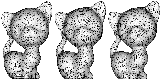
\includegraphics[width=0.9\textwidth]{figs/gcvt/comparison-kitten}\\
\begin{scriptsize}
\makebox[0.3\textwidth]{$\theta_{avg}=53.1$, $I=0.22$}
\makebox[0.3\textwidth]{$\theta_{avg}=55.1$, $I=0.13$}
\makebox[0.3\textwidth]{$\theta_{avg}=53.8$, $I=0.18$}\\
\makebox[0.3\textwidth]{$Q_{avg}=0.92$, $T=9.1s$}
\makebox[0.3\textwidth]{$Q_{avg}=0.94$, $T=354s$}
\makebox[0.3\textwidth]{$Q_{avg}=0.92$, $T=2109s$}\\
\end{scriptsize}
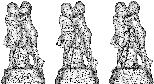
\includegraphics[width=0.9\textwidth]{figs/gcvt/comparison-scuplture}\\
\begin{scriptsize}
\makebox[0.3\textwidth]{$\theta_{avg}=52.1$, $I=0.25$}
\makebox[0.3\textwidth]{$\theta_{avg}=54.1$, $I=0.18$}
\makebox[0.3\textwidth]{$\theta_{avg}=53.3$, $I=0.22$}\\
\makebox[0.3\textwidth]{$Q_{avg}=0.90$, $T=7.2s$}
\makebox[0.3\textwidth]{$Q_{avg}=0.93$, $T=491s$}
\makebox[0.3\textwidth]{$Q_{avg}=0.92$, $T=3357s$}\\
\end{scriptsize}
\vspace{-0.1in}
\caption{Comparison with the RVD method~\cite{DBLP:journals/cgf/YanLLSW09} and the intrinsic CVT method~\cite{DBLP:journals/cad/WangYLXWGM015}.
 }
  \label{fig:OursRVDGVD}
\end{figure}


%------------------------------------------------------------------------
\begin{table*}[tbh]
\caption{Model complexity and runtime performance. $SS$: time (in seconds) for shell construction; $m$: the number of seeds; $T$: average time for each Lloyd iteration; $n$: the number of iterations;
 $I$: singularity ratio. }
% \vspace{-0.1in}
\begin{center}
\tabcolsep=0.11cm
\begin{tabular}{ccccccccccccc}
\hline
    Model & $d$ & $SS$(s) & \# of Sites & $m$ & $T$(s) & $n$ & $I$ & $Q_{min}$ & $Q_{avg}$ & $\theta _{min}$ & $\theta _{avg}$ & Time(s)\\
 \hline
    Sculpture    & 3    & 0.966    &   1.04 $\times$ $10^6$  & 3K & 0.064 & 100 & 0.25 & 0.639 & 0.907 & 36.1 & 52.4 & 7.2 \\
    Heptoroid      & 2    & 1.429    &   2.63 $\times$ $10^6$  & 9K & 0.138 & 120 & 0.24 & 0.624 & 0.902 & 35.3 & 51.9 & 19.5 \\
    Helix     & 2    & 1.212    &   4.4 $\times$ $10^5$  & 4K & 0.036 & 100 & 0.29 & 0.589 & 0.889 & 33.4 & 50.9 & 5.14 \\
    Pegaso       & 2    & 0.948    &   1.33 $\times$ $10^6$  & 8K & 0.063 & 150 & 0.26 & 0.600 & 0.894 & 31.5 & 51.3 & 10.6 \\
    Dinosaur     & 2    & 0.880    &   5.5 $\times$ $10^5$  & 4K & 0.025 & 160 & 0.28 & 0.636 & 0.894 & 30.2 & 51.2 & 4.8 \\
                 & 4    & 0.913    &   5.5 $\times$ $10^5$  & 1K & 0.046 & 170 & 0.31 & 0.602 & 0.900 & 30.6 & 51.8 & 9.2 \\
     Armadillo    & 2    & 0.944    &   1.26 $\times$ $10^6$  & 4K & 0.051 & 200 & 0.26 & 0.613 & 0.902 & 30.3 & 51.9 & 11.3\\
 \hline
\end{tabular}
\end{center}
\label{tab:Performancetable}
\end{table*}


%------------------------------------------------------------------------
\vspace{-0.5cm}
\section{Conclusion and Future Work}
\label{sec:conclusion}
  This paper presents a robust and efficient method for constructing isotropic meshes using Euclidean Distance Transform.
  Our algorithm constructs a narrow band space enclosing the input surface, in which 3D centroidal Voronoi tessellations and restricted Voronoi diagrams are computed.
  Our algorithm is fully parallel and memory-efficient,
  and it can construct the shell space with resolution up to $2048^3$ at interactive speed.
  Moreover, our method can process implicit surfaces, polyhedral surfaces and point clouds in a unified framework.
  Computational results show that our GPU-friendly isotropic meshing algorithm produces results comparable to state-of-the-art techniques,
  but runs significantly faster than the conventional CPU-based implementations.

   Our current implementation adopts a constant resolution to construct the shell space.
   This, however, is not optimal, since it is over-pessimistic for the regions with fairly flat geometry,
   and it may not be enough for the highly-curved.
   In the future, we will develop a geometry-aware algorithm for parallel constructing the shell space with adaptive resolution.
%-------------------------------------------------------------------------

\begin{figure}[tbh]
\centerline{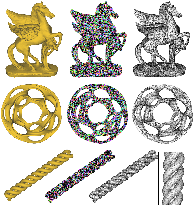
\includegraphics[width=0.9\linewidth]{figs/gcvt/models4}}
\vspace{-0.1in}
\caption{Experimental results. Images are rendered in high-resolution, allowing zooming in examination.}
  \label{fig:other models}
\end{figure}




